\documentclass{ufla}
\usepackage[portuges]{babel}
\usepackage[allbordercolors={1 1 1}, bookmarks=true, bookmarksnumbered=true,
		pdftitle={Uma ferramenta de e-commerce para elabora��o e compra de computadores com hardware customizado},
        pdfauthor={Igor Horta Corr�a},
        pdfsubject={Monografia},
        pdfkeywords={E-Commerce. Tecnologia da Informa��o. Extra��o de Dados. Minera��o de Dados.}]{hyperref}
\usepackage[latin1]{inputenc}
\usepackage[cmex10]{amsmath}
\usepackage{ae}
\usepackage{multirow}
\usepackage{color}
\usepackage{listings}
\usepackage{tabularx}
\usepackage[vlined,linesnumbered,titlenumbered,portuguese]{algorithm2e}
\usepackage[alf,abnt-etal-cite=3,abnt-etal-list=0,abnt-etal-text=plain,abnt-repeated-title-omit=yes,abnt-show-options=warn]{abntex2cite}
\usepackage{pslatex}

% Configuracao do listings
\lstset{ %
language=C++,                % choose the language of the code
basicstyle=\small\ttfamily,       % the size of the fonts that are used for the code
numbers=left,                   % where to put the line-numbers
numberstyle=\small,      % the size of the fonts that are used for the line-numbers
stepnumber=1,                   % the step between two line-numbers. If it is 1 each line will be numbered
numbersep=1ex,                  % how far the line-numbers are from the code
backgroundcolor=\color{white},  % choose the background color. You must add \usepackage{color}
showspaces=false,               % show spaces adding particular underscores
showstringspaces=false,         % underline spaces within strings
showtabs=false,                 % show tabs within strings adding particular underscores
frame=single,           % adds a frame around the code
tabsize=2,          % sets default tabsize to 2 spaces
captionpos=t,           % sets the caption-position to bottom
breaklines=true,        % sets automatic line breaking
breakatwhitespace=false,    % sets if automatic breaks should only happen at whitespace
keywordstyle=\color[rgb]{0,0,1},
commentstyle=\color[rgb]{0.133,0.545,0.133},
stringstyle=\color[rgb]{0.627,0.126,0.941}
}


\newcommand{\defs}[1]{\textsl{#1}}

\author{Igor Horta Correa}
\title{Uma ferramenta de \emph{e-commerce} para elabora��o e compra de computadores com \emph{hardware} customizado}
%\folhaaprovacao{Img/folha-de-aprovacao.pdf}
\date{2015}
\tipo{Monografia apresentada ao Colegiado do Curso de Sistemas de Informa��o, para a obten��o do t�tulo de Bacharel em Sistemas de Informa��o.}
\areaconcentracao{Sistemas de Informa��o}

\orientador{MSc. Renato Resende Ribeiro de Oliveira}
\coorientador{Dr. Denilson Alves Pereira}
\coorientadorbanca{Dr. Denilson A. Pereira}
\coorientadorbancainst{UFLA}
\bancaum{Dr. Ahmed A. A. Esmin}
\bancauminst{UFLA}
\bancadois{Dr. Raphael W. de Bettio}
\bancadoisinst{UFLA}
\defesa{24 de janeiro de 2016.}
\palchaves{E-Commerce. Tecnologia da Informa��o. Extra��o de Dados. Minera��o de Dados.}
\keywords{E-Commerce. Information Technology. Data Extraction. Data Mining.}


% Dados para ficha catalogr�fica
\fcautor{Correa, Igor Horta.}
\fcorientador{Renato R. R. de Oliveira}
% Tipo de material para ficha catalogr�fica
\fctipo{Monografia (gradua��o) -- Universidade Federal de Lavras, 2016.}
% dados para ficha catalogr�fica 
\fccatalogacao{1. Extra��o de dados da web. 2. E-Commerce. 3. Web. 4. Banco de dados. I. Universidade Federal de Lavras. I. T�tulo.}
% classifica��o de acordo com a CDD
\fccdd{CDD -- 004.6}


\hyphenation{Sistemas Informa��o Colegiado Curso Bacharel Universidade Federal Lavras Gradua��o}

% Aumente este numero para aumentar o espacamento no sum�rio
% entre os numeros das secoes e os titulos.
\scalenumwidth{1}

% Preguicoso :P
\sloppy

\begin{document}

\pagestyle{empty}
\dedic{
O presente trabalho
}

\thanks{
Agrade�o a.

Agrade�o tamb�m a.
}

\resumo{
Resumo da monografia
} % INCLUIR RESULTADOS

\resumoingles{
The english translation.
}

\listoffigures
\listoftables
\listofacronyms{
	\item[HTML] Hypertext Markup Language
	\item[JS] JavaScript
	\item[JVM] Java Virtual Machine
	\item[SGBD] Sistema Gerenciador de Banco de Dados
	\item[MVC] Model View Controller
	\item[XML] Extensible Markup Language
	\item[DOM] Document Object Mode
}
\tableofcontents

\pagestyle{ufla}

\section{INTRODU��O}
\label{sec:intro}

\subsection{Contextualiza��o e Motiva��o}

Com o advento da Internet, surgiu tamb�m uma nova esp�cie de com�rcio, o chamado \emph{e-commerce} ou com�rcio digital, que possui a vantagem de n�o limitar geograficamente o consumidor e disponibilizar para o mesmo um maior conjunto de lojas e produtos dispon�veis.
De acordo com a E-bit, as vendas no com�rcio eletr�nico em 2014 no Brasil continuaram crescendo e atingiram um resultado al�m do esperado. Segundo a mesma o faturamento do setor \emph{e-commerce} arrecadou com vendas o equivalente a R\$35,8 bilh�es. O que representa um crescimento de 24\% em rela��o a 2013, quando se vendeu um total de R\$28,8 bilh�es \cite{EBIT2015}. 


O n�mero de pedidos tamb�m aumentou, segundo a \cite{EBIT2015}, o aumento deste em 2014 foi de 17\% em rela��o ao ano
anterior, chegando a 103,4 milh�es. Em 2013 foram 88,3 milh�es de encomendas de bens de consumo via Internet. Em 2015, espera-se que o n�mero de encomendas seja 19\% maior, chegando a 122,9 milh�es.


Com o aumento dos requisitos m�nimos para se utilizar jogos e programas atuais e com o aumento de poss�veis combina��es de pe�as de computadores, a tarefa de customizar seu pr�prio computador para executar fun��es especificas se torna cada vez mais dif�cil.


Tendo como base o crescente sucesso e procura do com�rcio eletr�nico e consequentemente o aumento de \emph{web} sites de \emph{e-coomerce}, este trabalho prop�e um sistema para facilitar a tarefa de customizar seu pr�prio computador. Tal sistema utilizara t�cnicas de extra��o de dados para obter pre�os e informa��es sobre diversas pe�as de computadores de diferentes sites especializados em comercio eletr�nico. Com tais informa��es dispon�veis o sistema proposto ir� disponibilizar diversos recursos como compara��o de pre�os entre pe�as e auxilio na customiza��o de computadores visando o melhor custo benef�cio. 



\subsection{Objetivos Gerais e Espec�ficos}
O objetivo geral deste trabalho � uma aplica��o web que auxilie o usu�rio a comprar e montar seu computador personalizado, tal aplica��o possuir� o recurso de compara��o de pre�os de pe�as de computadores das principais lojas de \emph{e-commerce} atuais.

Visando atingir este objetivo geral, os objetivos espec�ficos s�o definido a seguir:
\begin{itemize}
\setlength{\itemsep}{-0.3ex}
\item Desenvolver um algoritmo eficiente que seja capaz de coletar informa��es de produtos em diferentes sites de e-commerce.
\item Desenvolver um prot�tipo de interface para aplica��o.
\item Modelar o banco de dados da aplica��o.
\end{itemize}



\subsection{Metodologia}
Breve descri��o da metodologia que foi utilizada...



\subsection{Organiza��o do Trabalho}
O trabalho est� organizado da seguinte forma, na Se��o~\ref{sec:review} ser� apresentado um referencial te�rico acerca dos conceitos utilizados. Na Se��o~\ref{sec:metod} ser� apresentada a metodologia do trabalho desenvolvido. Na Se��o~\ref{sec:results} ser�o apresentadas as simula��es computacionais realizadas e os resultados obtidos. As conclus�es e os trabalhos futuros ser�o apresentadas na Se��o~\ref{sec:conclusion}.


\section{REFERENCIAL TE�RICO}
\label{sec:review}

% 
%%% 
%%% 
%%% 
%%% 
%


\subsection{Hypertext Markup Language (HTML)}
O \emph{Hypertext Markup Language} (HTML) � uma linguagem de marca��o utilizada para descrever documentos da web (\emph{websites}). Linguagem de marca��o � um conjunto de \emph{tags} (palavras reservadas da linguagem) e regras que ao serem aplicados em um arquivo de texto prov�m informa��es sobre como o documento deve ser editado, formatado, exibido e impresso.


A \emph{World Wide Web} sempre utilizou o HTML como linguagem de marca��o. Inicialmente o HTML foi desenvolvido para suprir a necessidade de descrever semanticamente documentos acad�micos. Entretanto ao passar dos anos este sofreu significativas adapta��es e melhorias para suportar novos tipos de documentos.

Em HTML, as \emph{tags} normalmente s�o utilizadas em duplas, onde cada uma indica o in�cio e fim do texto que est� sendo demarcado, como por exemplo:

\begin{center}
 \texttt{<title>Ol� mundo</title>}
\end{center}

Ao interpretar este trecho de HTML, o navegador do usu�rio que est� acessando o documento ir� entender que o t�tulo da p�gina deve ser ``Ol� mundo''.

A Figura~1 mostra um exemplo de um documento escrito em HTML. Segundo \citeonline{w3c_html5} o HTML � dividido em 2 partes principais, \emph{head} (cabe�alho) e \emph{body} (corpo).
O t�tulo do documento juntamente com demais informa��es sobre o mesmo ficam dentro da \emph{tag} \texttt{<head>}. Dentro da \emph{tag} \texttt{<body>} se encontra o conte�do (corpo) do documento. J� as \emph{tags} \texttt{<h1>}, \texttt{<h2>}, \texttt{<h3>} representam t�picos no documento, onde \texttt{<h1>} � um elemento mais importante que \texttt{<h2>} e que \texttt{<h3>}. Os navegadores normalmente exibem os t�picos mais importantes com fontes maiores do que t�picos menos importantes.
A Figura~2 apresenta a interpreta��o deste exemplo pelo navegador \emph{Google Chrome}.

  
\begin{figure}[!h!t!b]
\centering
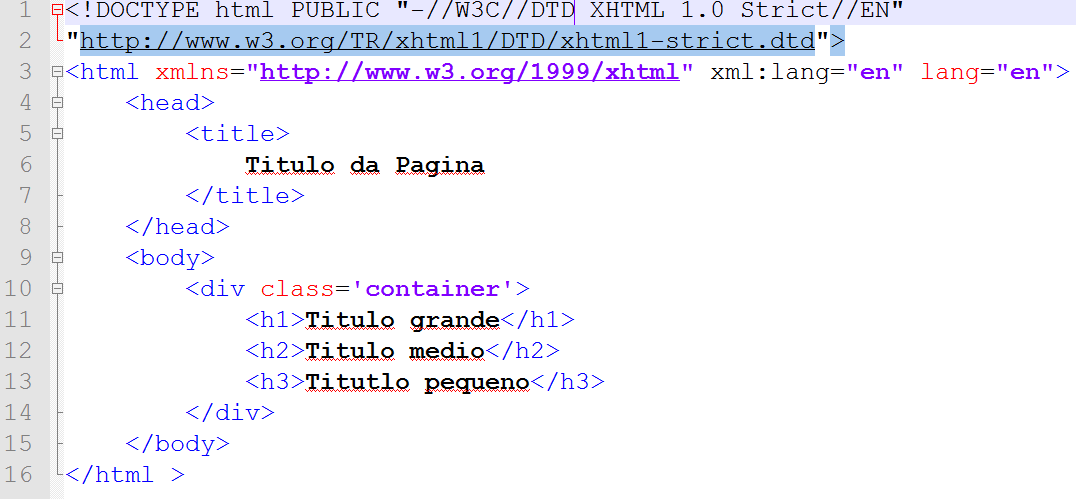
\includegraphics[width=\columnwidth]{img/imagem1-tcc}
\caption{Exemplo de documento em HTML.}
\end{figure}


\begin{figure}[!h!t!b]
\centering
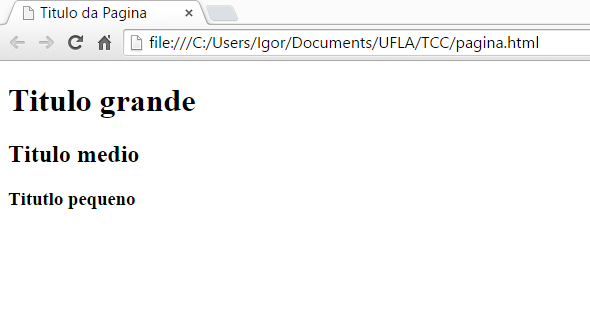
\includegraphics[width=8cm]{img/imagem4-tcc}
\caption{Interpreta��o de c�digo HTML pelo browser Google Chrome.}
\end{figure}

% TODO Horta, seria interessante no final desta subse��o que voc� explicasse que as p�ginas
% das lojas de e-commerce s�o escritas em HTML e que para voc� extrair as informa��es de que precisa voc� precisar ler, interpretar e processar os c�digos HTML
% das lojas de e-commerce.
% Seria bom complementar tamb�m dizendo que o sistema web que ser� desenvolvido apresentar� as informa��es utilizando HTML tamb�m.



%%
%%%%
%%%%%%
\subsection{Javascript}
O \emph{Javascript} � uma linguagem de programa��o \emph{script} que � muito utilizada atualmente para cria��o de p�ginas da web din�micas. Tamb�m � muito utilizada para constru��o de aplica��es web. Isso se deve ao fato de os navegadores modernos suportam por padr�o o uso dessa linguagem pelos \emph{websites}.

Segundo \cite{EcmaScript} linguagem de \emph{script} � uma linguagem de programa��o usada para manipular, customizar e otimizar recursos j� existentes em um programa. Em tais sistemas, funcionalidades �teis j� s�o disponibilizadas atrav�s de uma interface para o usu�rio. A linguagem de \emph{script} � um mecanismo para disponibilizar tais funcionalidades tamb�m para o controle da aplica��o.


De acordo com \cite{flanagan2002javascript}, Javascript � uma linguagem de \emph{script} com suporte a orienta��o a objetos. Na programa��o orientada a objetos implementa-se um conjunto de classes que definem os objetos presentes na aplica��o. Cada classe determina o comportamento (definido nos m�todos) e estados poss�veis (atributos) de seus objetos, assim como o relacionamento com outros objetos.


Quando utilizada no \emph{client-side} (lado do cliente), o Javascript permite que conte�do execut�vel seja adicionado �s p�ginas \emph{web}, o que possibilita que estas p�ginas interajam com o usu�rio, controlem o navegador e criem conte�do HTML dinamicamente.


\begin{figure}[!h!t!b]
\centering
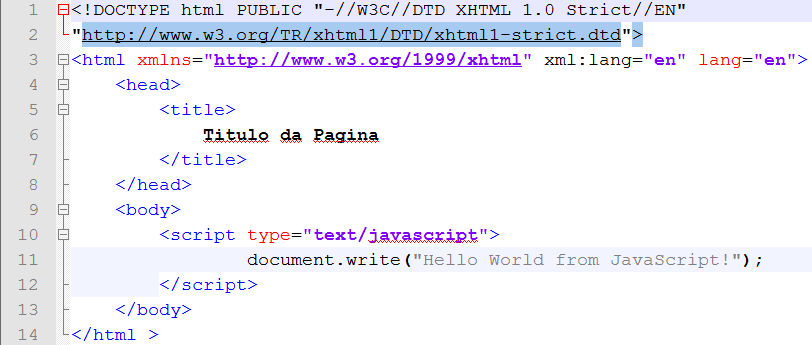
\includegraphics[width=\columnwidth]{img/imagem5-tcc}
\caption{C�digo em HTML com trecho em Javascript.}
\end{figure}

% TODO Lembrete, NUNCA pode se separar o sujeito do verbo com v�rgula/ponto. Ex:
% ERRADO: A Figura~3, apresenta...
% CORRETO: A Figura~3 apresenta...
% Figura � o sujeito, apresenta � o verbo.
A Figura~3 apresenta um documento em HTML que possui um trecho de c�digo em Javascript. Este trecho se encontra dentro da \emph{tag} \texttt{<script>}, isso indica ao navegador que este trecho trata-se de um c�digo em Javascript.
Na linha 11 pode-se observar a chamada da fun��o \emph{write} do objeto \emph{document}. Esta fun��o tem como objetivo adicionar dinamicamente um texto ou conte�do qualquer � p�gina que est� sendo exibida pelo navegador.

% TODO Complementar dizendo que Javascript � utilizado na maioria dos sites de e-commerce.
% Citar o poss�vel problema para extra��o de dados caso os sites de e-commerce insiram os pre�os dos produtos dinamicamente via Javascript.
% Pode citar a monografia do Leandro e observar que o c�digo que ele desenvolveu n�o dava suporte � extra��o dos pre�os que isso ocorria.
% Cita que no presente trabalho este problema ser� tratado e forma de solucion�-lo ser�o propostas.
% Outra coisa, diga que v�rias partes do sistema web que est� sendo proposto ser�o feitas com Javascript.




%
%%
%%%%
%%%%%%
\subsection{PhantomJS}
Phatomjs � um navegador \emph{opensource} \emph{webkit}, program�vel em Javascript que possui suporte para diversos padr�es web como: manipula��o da DOM,  seletores CSS, JSON, Canvas e SVG.
Com o Phatomjs se � poss�vel:

\begin{itemize}
\setlength{\itemsep}{-0.3ex}
\item Realizar testes unit�rios para aplica��es web.
\item Carregar, analisar e renderizar p�ginas web.
\item Obter screenshots de websites.
\end{itemize}

O c�digo apresentado na figura 4,  associa uma inst�ncia da classe webpage do PhantomJS a uma vari�vel chamada page, a partir de ent�o
a fun��o open � chamada, esta fun��o faz uma requisi��o ao site passado como par�metro, no caso 'http://phatomjs.org/',se a requisi��o for um sucesso uma c�pia da imagem renderizada pelo navegador PhantomJS e criada.

\begin{figure}[!h!t!b]
\centering
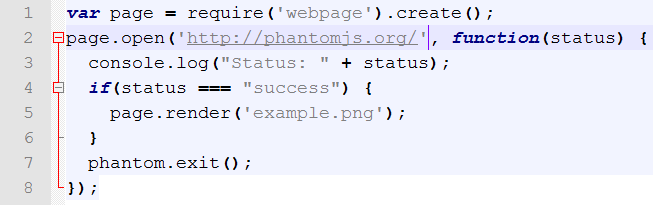
\includegraphics[width=7.5cm]{img/imagem2-tcc}
\caption{Exemplo de c�digo em Javascrpit que sera executado pelo phatomjs}
\end{figure}

A figura a seguir � a imagem gerada pelo c�digo em Javascript

\begin{figure}[!h!t!b]
\centering
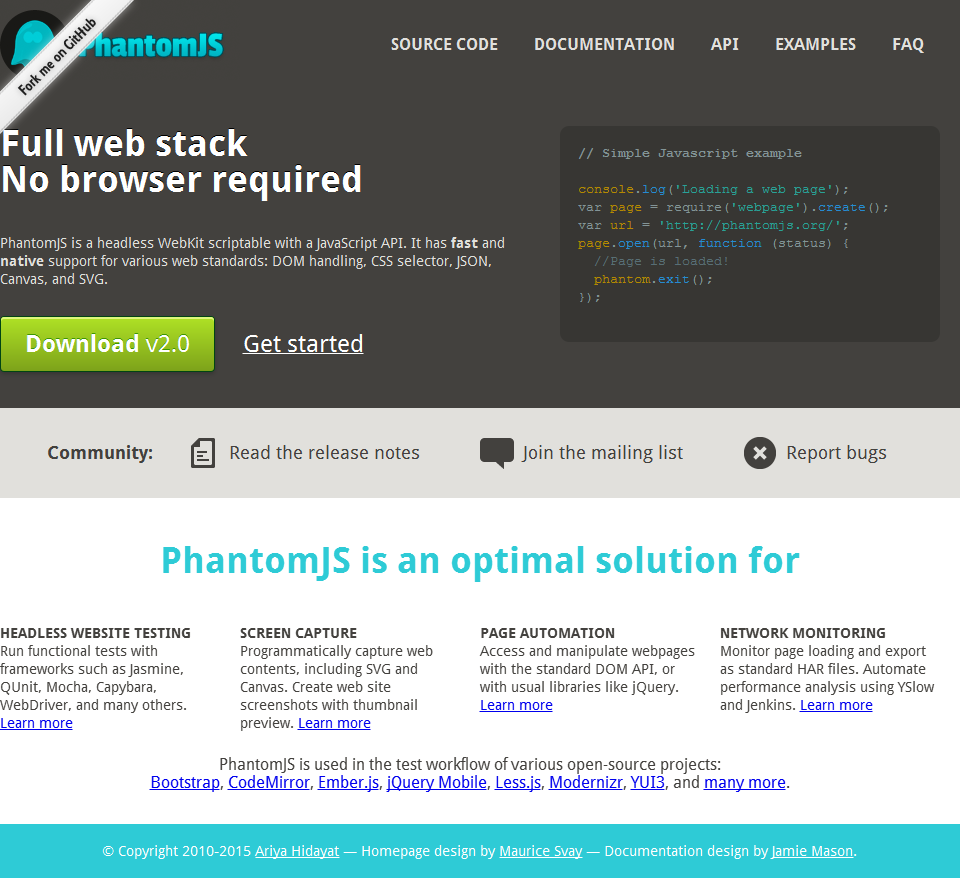
\includegraphics[width=7.5cm]{img/example}
\caption{Imagem gerada ap�s a execu��o do c�digo em Javascript}
\end{figure}


%
%
%
%%%%%%%%%%
\subsection{Java}
A linguagem de programa��o Java  come�ou a ser desenvolvida em 1991 com a finalidade de ser utilizada em dispositivos eletr�nicos inteligentes, porem com  o crescimento exponencial da \emph{World Wide Web} em 1993, os engenheiros da \emph{Sun Microsystems} notaram o potencial da linguagem para aprimorar a funcionalidade de servidores \emph{web} e a adaptou para estas fun��es.

A linguagem Java � orientada a objetos e possui o diferencial de ser interpretada, ou seja, diferentemente de linguagens como c e c++ em que seus c�digos s�o diretamente transformados em c�digos de maquinas quando compiladas, o java possui seu c�digo transformado em uma linguagem intermediaria, esta � ent�o interpretada em tempo de execu��o por um programa chamado \emph{Java Virtual Machine}.Como resultado, Java pode muitas vezes atingir um n�vel de efici�ncia que � inating�vel com int�rpretes tradicionais.


Segundo \cite{roberts2013art} As caracter�sticas principais do Java incluem o fato dela ser f�cil de ser programada sem a necessidade de treinamento extensivo do desenvolvedor. Em Java estes desenvolvedores tem acesso a diversas bibliotecas que oferecem uma s�rie de  recursos j� implementados tais como opera��es de entrada e sa�da, \emph{interface} para redes e recursos gr�ficos. Por ser uma linguagem interpretada,  uma outra vantagem � o fato dela possuir uma verifica��o de erros em tempo de execu��o.



%%
%%%%
%%%%%%
\subsection{MySQL}
SGBD ou (sistema gerenciador de banco de dados), � um conjunto de programas que tem como objetivo armazenar, alterar, apagar e proteger informa��es de uma base de dados. Estes s�o bastante uteis em aplica��es web, por permitirem que as informa��es sejam armazenadas e utilizadas automaticamente.

 
Banco de dados armazenam informa��es sobre objetos distintos, entidades, associa��es ou ate mesmo sobre o relacionamento entre estas entidades. Como por exemplo, um banco para vendas pode guardar informa��es sobre produtos, clientes e vendas. Neste caso produtos e clientes s�o entidades enquanto vendas � um relacionamento entre cliente e produto.

No modelo de dados relacional os dados s�o percebidos pelos usu�rios como tabelas, onde cada coluna armazena um tipo de dados que podem ser de diversos tipos diferentes como num�ricos, reais, texto e etc. Cada linha desta tabela representa uma inst�ncia.


Na figura 6: podemos ver como os dados s�o representados em um modelo relacional, a coluna ClienteID representa o identificador do cliente este n�mero deve ser �nico, a segunda coluna representa o nome e a terceira o telefone celular de cada uma das linhas correspondentes.

\begin{figure}[!h!t!b]
\centering
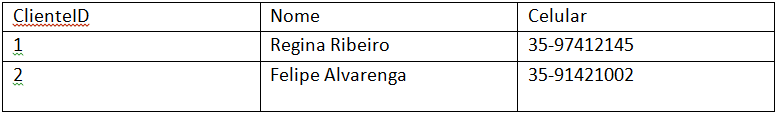
\includegraphics[width=7.5cm]{img/imagem7-tcc}
\caption{Exemplo de uma tabela de uma banco de dados relacional.}
\end{figure}

 
O MySQL segundo \cite{tahaghoghi2006learning} � um popular SGBD relacional \emph{openSource}, que se destaca dos demais concorrentes por uma s�rie de motivos, dentre elas podemos ressaltar: seu tamanho e velocidade, o MySQL funciona bem ate mesmo nos hardwares mais modestos, a velocidade com que ele consegue recuperar informa��es foi fator fundamental para torna-lo o SGBD favorito em diversas organiza��es. Outro fator muito importante para sua aceita��o � a sua f�cil instala��o que pode ser realizada sem grandes dificuldades e com pouca configura��o 
 

%%
%%%%
%%%%%%
\subsection{Hibernate}
Segundo \cite{5071809}, enquanto o paradigma relacional � um modelo extremamente comum em populares  banco de dados do mercado, a programa��o orientada a objetos tamb�m � extremamente comum em aplica��es atuais, logo a combina��o entre estas tecnologias de diferentes paradigmas se torna inevit�vel.  Enquanto o modelo relacional trata os dados como tabelas, o modelo orientado a objetos os representa como um conjunto de objetos, tamanha diferen�a em como os dados s�o representados geram uma s�rie de problemas em aplica��es que utilizam SGBDS relacionais e linguagens orientadas a objeto.


Como uma alternativa para este problema, algumas ferramentas de mapeamento objeto/relacional(MOR) foram criadas, dentre essas destaca-se o Hibernate

O Hibernate � um \emph{framework}(ferramenta) de alta performance para mapeamento objeto/relacional em java. Este \emph{framework} associa classes em java a tabelas do banco de dados. Ele tamb�m permite abstrair c�digo sql em objetos java.
Etre as diversas vantagens do Hibernate podemos ressaltar a facilidade em alterar formatados das tabelas, simplesmente alterando as classes java que as representam.


%%
%%%%
%%%%%
\subsection{VRaptor}
\emph{Model View Controller}(Modelo Vis�o controlador) � um padr�o de arquitetura de \emph{software}, que separa a aplica��o em tr�s partes. O modelo (\emph{model}) representa os dados da aplica��o e suas respectivas regras de neg�cios. A vis�o (\emph{view}) pode ser qualquer sa�da de representa��o dos dados.O controlador(\emph{controller}) faz a media��o da entrada, preparando-a em comandos para o modelo ou vis�o.
O objetivo principal do MVC � trazer para aplica��o reusabilidade de c�digo e separa��o de conceitos.


O Vraptor � um \emph{framework} \emph{MVC} de c�digo livre focado em gerar alta produtividade, foi designado para dar suporte ao desenvolvimento de \emph{websites} din�micos bem como aplica��es \emph{web} que fazem uso do modelo \emph{MVC}. Tem como objetivo poupar trabalho do desenvolvedor, mantendo-o focado nas suas atividades principais.
De acordo com \cite{cavalcanti2014vraptor}, com o Vraptor  � f�cil aplicar as melhores
pr�ticas de orienta��o a objetos, j� que este n�o imp�e restri��es no design das suas classes. � tamb�m um dos frameworks mais extens�veis em java, pois praticamente todos seus comportamentos podem ser sobrescritos com pouco c�digo, sem a necessidade de configura��es em \emph{XML}.Al�m disso, � um \emph{framework} que  deixa seus usu�rios totalmente livres para escolher sua camada de visualiza��o.  
Dentre as diversas vantagens citadas acima, podemos destacar o fato do Vraptor ser um \emph{framework} nacional com ampla documenta��o em portugu�s.
\section{METODOLOGIA}
\label{sec:metod}

\subsection{Extra��o de dados sobre produtos}

\cite{alonso2015agente} realizou um estudo sobre extra��o de pre�os em sites de \emph{e-commerce}. Neste trabalho foi desenvolvido um agente de \emph{Shopping Comparison} que utilizava padr�es em documentos HTML para obter produtos e seus respectivos atributos.Por�m este estudo possu�a o ponto deficiente de n�o conseguir obter informa��es de \emph{websites} que utilizam a linguagem Javascript para exibir o pre�os dos produtos assincronamente, o que � uma pr�tica comum em sites atuais.

O presente trabalho tratar� os pontos deficientes do estudo de \citeonline{alonso2015agente}, e tamb�m abordara outras funcionalidades da aplica��o em si.

Um dos recursos do sistema proposto � proporcionar a compara��o de pre�os de pe�as de computador entre diversas lojas de \emph{e-commerce}, para se obter a informa��o de cada pe�a com seus respectivos pre�os e vendedores o sistema utilizara de um algoritmo de extra��o de dados. Tal algoritmo sera desenvolvido em Javascript e ser� executado utilizando o PhantomJS.
Os dados que deveram ser extra�dos dos \emph{websites} voltados para o \emph{e-commerce} s�o:


\begin{itemize}
\setlength{\itemsep}{-0.3ex}
\item nome do produto.
\item link da imagem do produto.
\item pre�o do produto.
\item descri��o do produto.
\item link para a compra do produto.
\end{itemize}


As informa��es do produto como nome, \emph{link} da imagem, pre�o, \emph{link} para a compra ser�o necess�rias para identificar o produto, exibir sua imagem e manter informa��es sobre o vendedor.

Para se obter tais informa��es ser� criado um \emph{script} que adotara a seguinte estrat�gia: obter a �rvore DOM do \emph{website} utilizando fun��es disponibilizadas pelo phatomJS e ai ent�o utilizando a DOM juntamente com seletores CSS o algoritmo ira buscar pelo car�cter \$ pois o mesmo denota pre�o, ao encontra-lo  analisara os elementos pr�ximos do mesmo n�vel em busca de uma imagem e nome do produto. Se tais elementos forem localizados, o algoritmo ent�o conseguiu identificar um poss�vel produto.Para confirmar que o item obtido � o que se procura, o algoritmo ira \"subir\" alguns n�veis na arvore DOM e ent�o procurar nos elementos pr�ximos por itens semelhantes, se uma sequ�ncia de produtos semelhantes forem encontrados, o algoritmo ent�o ira armazenar estes itens em uma lista e os enviara para a aplica��o.


\subsection{Persist�ncia dos dados}

O sistema proposto possuir� 2 tabelas essenciais no banco de dados, sendo a primeira de lojas, que conter� informa��es sobre as lojas de \emph{e-commerce}, a segunda tabela contar� com informa��es sobre os produtos e ser� preenchida com os dados obtidos por meio do algoritmo de extra��o de dados, tais dados ser�o tratados e ter�o sua integridade testada antes de serem salvos.

\begin{figure}[!h!t!b]
\centering
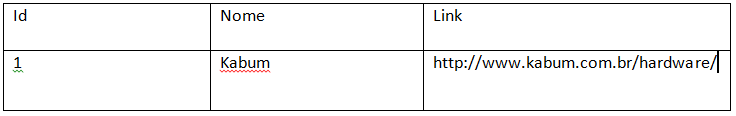
\includegraphics[width=\columnwidth]{img/imagem8-tcc}
\caption{Exemplo de uma tabela de lojas do banco de dados.}
\end{figure}



\begin{figure}[!h!t!b]
\centering
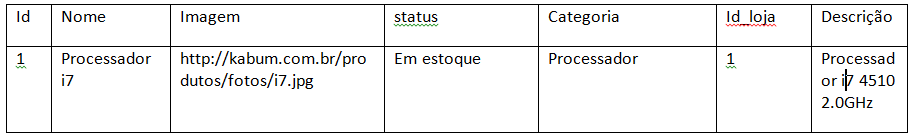
\includegraphics[width=\columnwidth]{img/imagem9-tcc}
\caption{Exemplo de uma tabela de produtos de um banco de dados.}
\end{figure}

A figura~7 representa uma tabela de lojas no banco de dados, tal tabela conter� o nome,\emph{link} para o site da loja e id de cada empresa que ter� seus dados extra�dos.

A figura~8 representa uma tabela de produtos no banco de dados, esta tabela ira conter informa��es como: id,nome,imagem,status,categoria,descri��o e um identificador que informara a qual loja este produto pertence.


\subsection{Listagem de produtos com compara��o de pre�os}

Com os dados extra�dos de diferentes lojas de \emph{e-commerce} voltadas para o com�rcio de hardware, sera poss�vel a implementa��o de uma interface \emph{web} que auxilie ao usu�rio na montagem do pr�prio computador personalizado. tal interface sera implementada utilizando-se as linguagens HTML,Javascript e CSS. 


Nela o usu�rio ter� acesso a diferentes tipos de pe�as de computadores, o sistema destacar� a pe�a mais barata de cada categoria e seu respectivo vendedor.



\section{RESULTADOS E DISCUSS�O}
\label{sec:results}


\subsection{Cronograma}
1 - Estudar sobre algoritmos de detec��o de padr�es em p�ginas HTML (1 m�s)

2 - Desenvolver um algoritmo eficiente para reconhecimento de padr�es em HTML, que trate 
altera��es na p�gina com Javascript (2 meses)

3 - Desenhar e planejar as telas da aplica��o (15 dias)

3 - Modelagem do banco de dados para a aplica��o (15 dias)

4 - Implementa��o do \emph{back-end} da aplica��o (1 m�s)

5 - Implementa��o do \emph{front-end} da aplica��o (1 m�s)

\subsection{Resultados Esperados}

Ao final deste trabalho espera-se um algoritmo que seja capaz de extrair pre�os e demais informa��es de pelo menos 5 sites de \emph{e-commerce} diferentes, sendo que pelo menos 2 deles utilizem a linguagem Javascript para atualizar as informa��es dos produtos assincronamente.


Tamb�m espera-se um prot�tipo de uma aplica��o \emph{web} que utilize os dados obtidos pelo algoritmo de extra��o de dados. Tal aplica��o deve ter como objetivo comparar os pre�os dos produtos obtidos pelo algoritmo.
\section{CONCLUS�O E TRABALHOS FUTUROS}
\label{sec:conclusion}


%\vfill\null\newpage
\renewcommand{\baselinestretch}{1.0}
\bibliographystyle{abntex2-alf}
\bibliografia{sections/refs}

\end{document}
